\chapter{Background}
\begin{quote}
"Jung states a Man cannot stand a meaningless life" (C Jung) 
\end{quote}

\newpage
\begin{figure}[h!]
\begin{center}
\includegraphics[scale=.25]{../eps/In_through_the_background.eps}
\caption{In through the background}
\label{label}
\end{center}
\end{figure}

\newpage
Before I start my inquiry, I want to orient you the reader and provide a small window illustrating the complexity of what mandalas can pose and why I hold drawing mandalas so dear to my heart. 

I sat down to reflect on the mandalas I have kept over the years and one stood out for me. I sat with this mandala which I produced in 2005 and was astounded by the message it had for me 10 years after producing it and I still remain fascinated by what it might continue to teach me in the future. I continue to be curious in particular about the power of mandalas and what the symbols represents as well as what resonates for me now. 

I explored two mandalas which were created 10 years apart, but remarkably have a connection and seem to be unified.   

The following mandala I drew on the 22 of November 2005 (which was the third year out of the twelve years my former partner and I were together) I drew this mandala in response to a dream amplification: 

\begin{figure}[h!] 
\begin{center}
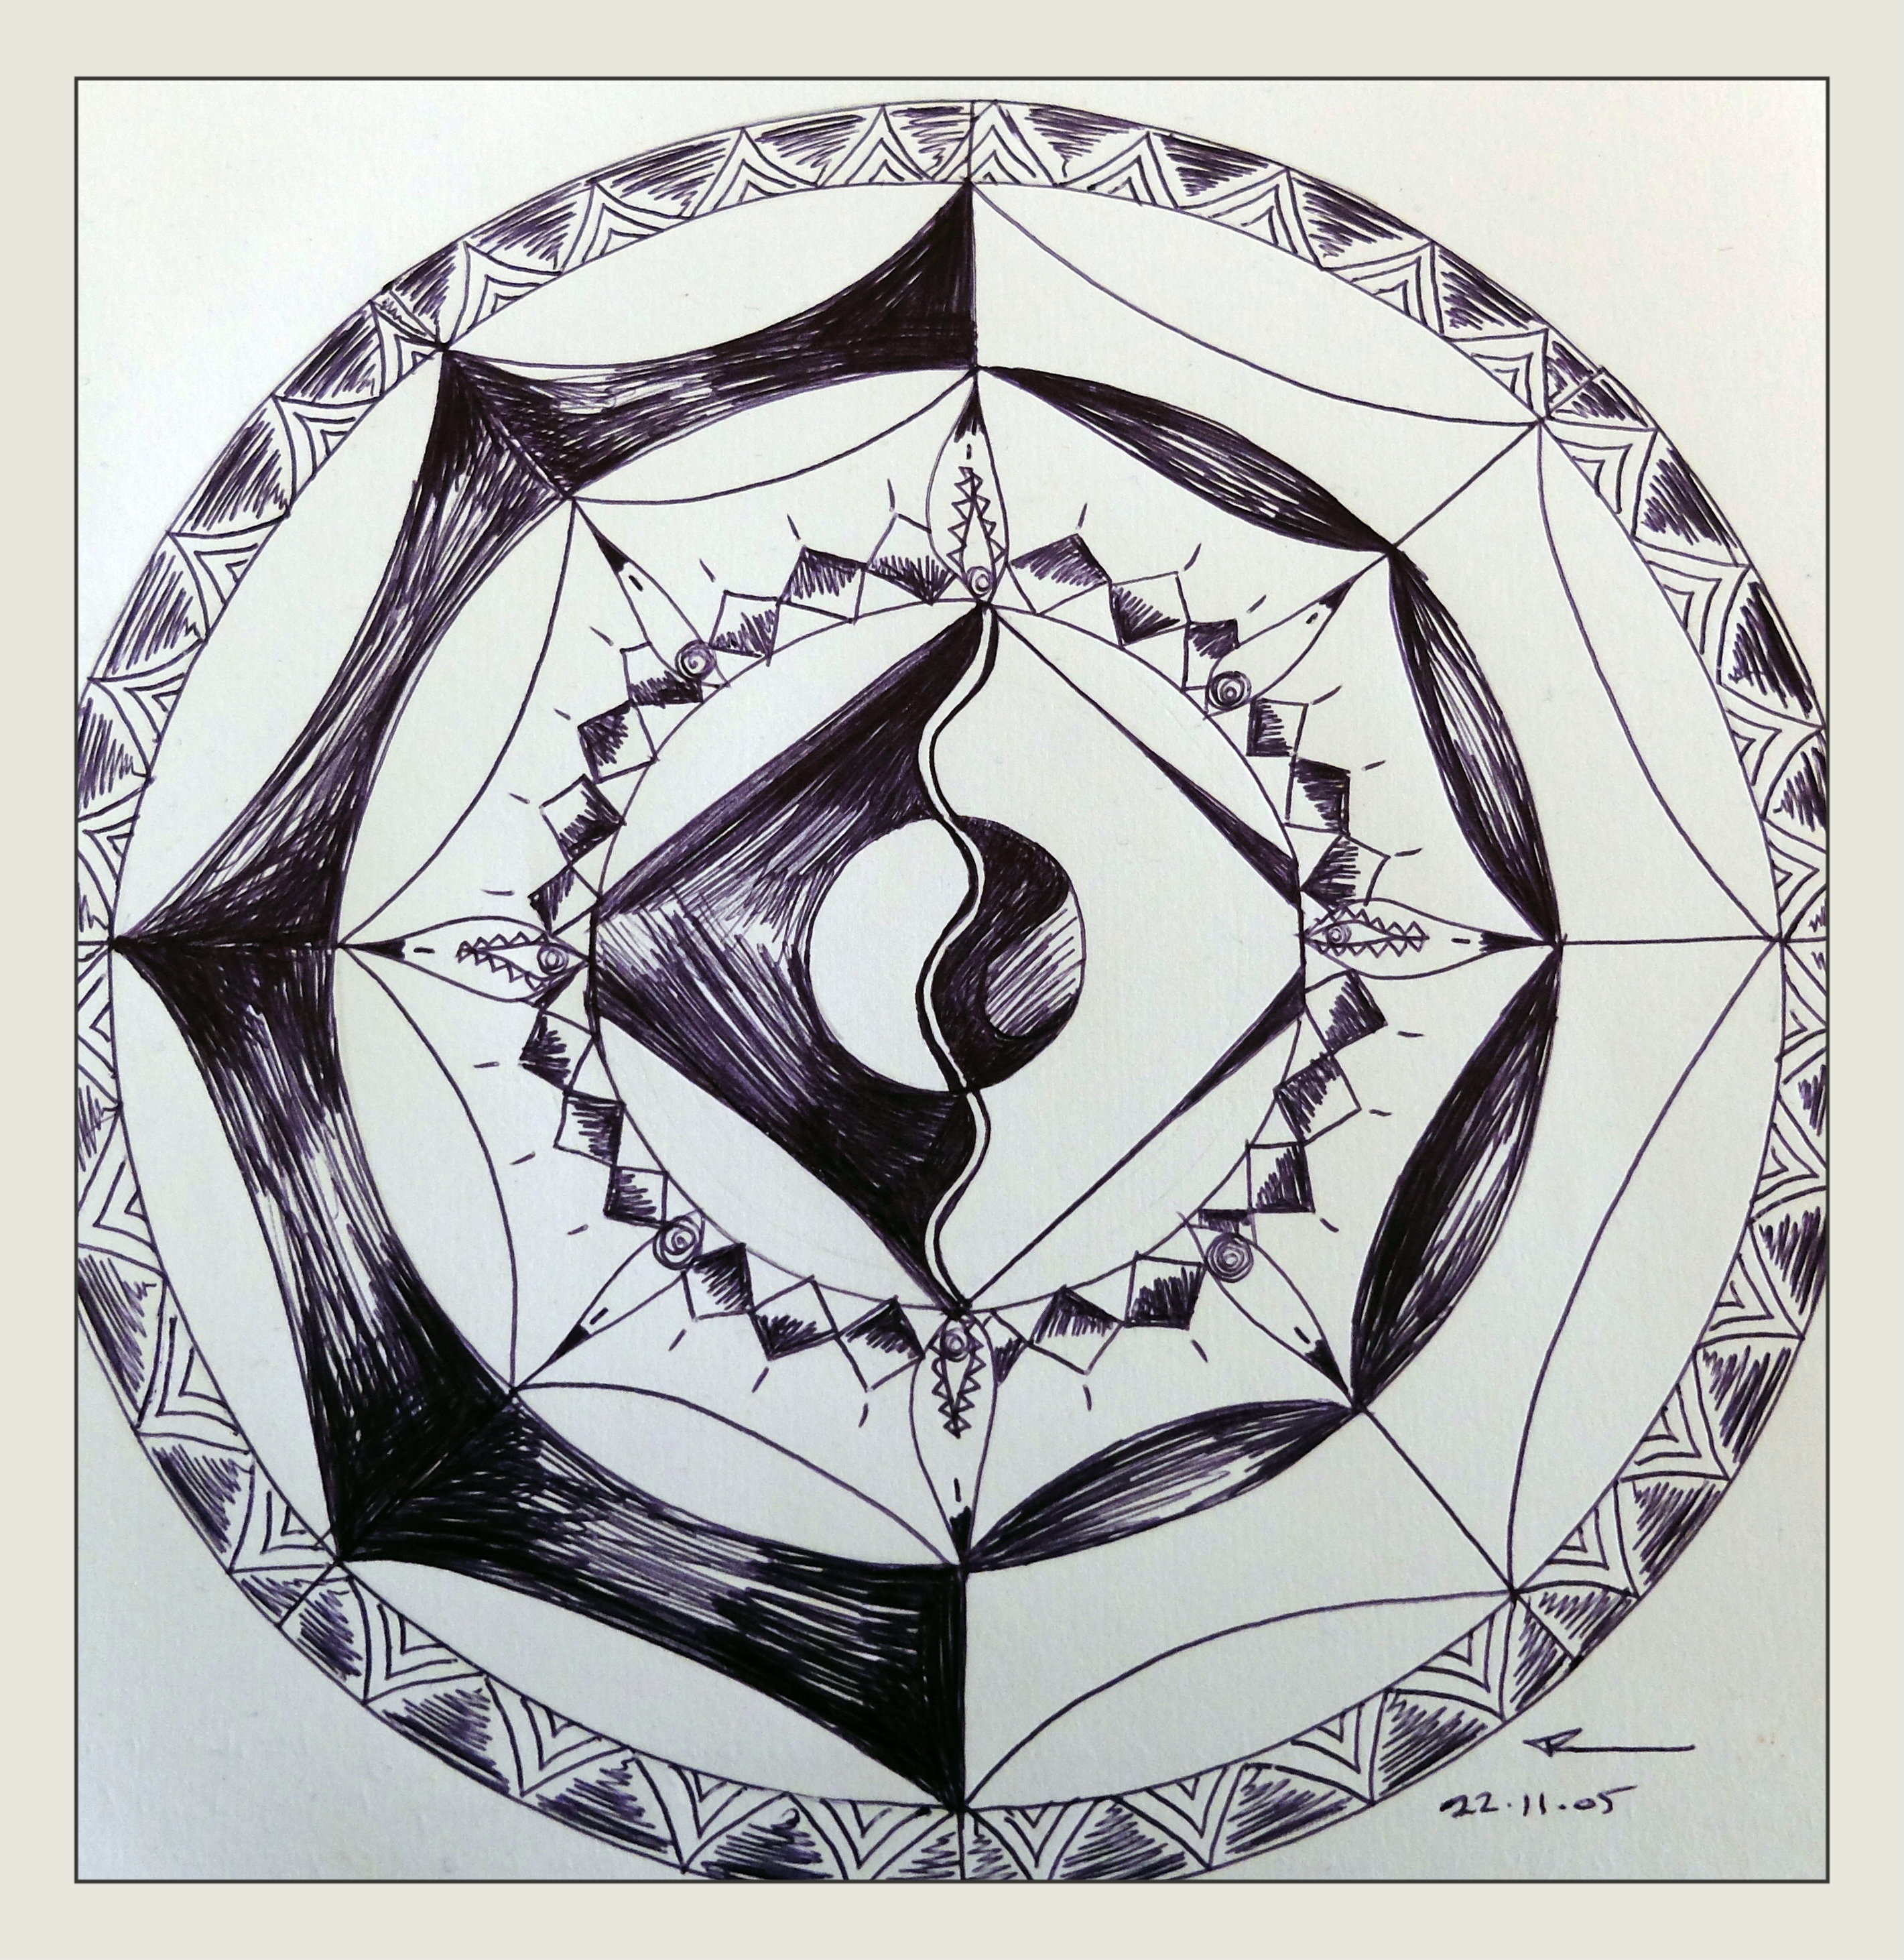
\includegraphics[scale=.1]{../eps/2005_m.eps}
\caption{2005 Mandala}
\label{label}
\end{center}
\end{figure}

%FIGURE 2-2005 MANDALA (try and get this up in this placement 

And wrote in my journal: \newline 

I have many dreams where we have broken up, as he has cheated on me, however I never thought he would actually cheat in real life. I feel that this dream is an indication of my fear of abandonment. We have been together for 3 years. He has never wanted to comment on our future which bothers me as it poses the question- When will he break up with me? Perhaps my ego is trying to balance my relationship and my emotions. I feel a lack of attention from him, not being able to ease my emotions about being together and not knowing when he might pull the rug from under me. I also feel my dream is also trying to communicate that I need to break away from a situation or any bad habits that I may have. As well as being balanced within myself and accept myself and stop with the self-deprivation.  

It is amazing that 10 years after I produced this mandala in 2005, my former partner did pull the rug from under me. He ended our relationship in 2014 abruptly without warning. He withdrew and disappeared to never say another word to me. I still remember how I felt in the dreams I had when he broke up with me. All those years later, when he did end our relationship, he behaved exactly like in my dreams. He was cold, empty, no compassion and had totally withdrawn. The only thing he revealed was that he felt lost and did not know what he wanted. I, on the other hand, had very clear goals; I wanted to complete my masters and to start a family with him. But after 12 years he was just as confused when I met him regarding what his aspirations were. I was attracted to his intelligence, his many talents and his beautiful blue eyes. He was my best friend and lover for 12 years and never spoke about being unhappy in our relationship, but at the same time he never commented on how he saw our future, even when we decided to get engaged in late 2013. 

Reflecting on the phrase of pulling the rug from under me, I have only now been able to understand the significance of this symbolic rug. It now makes perfect sense why I felt it was so important for me to keep the beautiful rug we bought in India. We did not have many possessions but the rug was the only thing that I yearned for when we went our separate ways. I felt lost when he left as it was excruciating and so sad that he chose to walk away and vanish. However, in my grief, I remained grounded and I never lost sight of who I was. Thus, it was invaluable for me to put my own feet on this beautiful soft rug and not get caught up in my self doubt around the questions why he left.


\begin{figure}[htbp]
\begin{center}
\includegraphics[scale=.2]{../eps/My_rug_.eps}
\caption{MY RUG!}
\label{label}
\end{center}
\end{figure}


Fast forward to the 8th of August 2015 to intensive three class for the MIECAT Masters program; after exploring my embodiment, I intuitively created a mandala which served as my new mantra. 



%FIGURE 4-MANDALA MANTRA
%FIGURE 5- DEFFINITION OF THE MANDALA MANTRA
%Get better picture and size

After my former partner revealed he wanted to separate, I woke up with the word reciprocity stuck in my head which has evidently stayed implanted in my body. As soon as I drew this wiggled line, I knew it represented reciprocity and balance for me. This wiggled line is similar to the shape of an 'S'. The wiggled shape is going through five different coloured circles, which are the same on either side of the wiggled line. They overlap each consecutive circle which is encompassed within a large circle. Each of these circles represent qualities I desire in an intimate relationship. 

They are as follows:
\begin{itemize}
\item Affection (white)
\end{itemize}

\begin{itemize}
\item Affirmation (red)
\end{itemize}

\begin{itemize}
\item Connection (green)
\end{itemize}

\begin{itemize}
\item Acknowledgment (yellow)
\end{itemize}

\begin{itemize}
\item and for the both of us to be Grounded (brown)
\end{itemize}

    
To my surprise this wiggled line is also similar to the centre of the mandala I drew all those years earlier in 2005, although in this early mandala this wiggled line is in the opposite direction. In the 2015 mandala the wiggled line has two different colours- red and green that slightly overlap each other in the centre of the line. In 2005 there is only black and white. This is quite interesting as in the past I looked at the world with a very black and white mentality but now I can see the world has so many more colours that blend into each other. It is refreshing to be able to appreciate their ever shifting elements and not be stuck in this fixed terminology. 



%FIGURE 6- 2015 MANDALA MANTRA
             		

%FIGURE 7- MANDALA 2005

Take a double exposure picture of these two mandalas

